%!TEX TS-program = xelatex
\documentclass[]{friggeri-cv}
\usepackage{afterpage}
\usepackage{hyperref}
\usepackage{color}
\usepackage{xcolor}
\hypersetup{
    pdftitle={},
    pdfauthor={},
    pdfsubject={},
    pdfkeywords={},
    colorlinks=false,       % no lik border color
   allbordercolors=white    % white border color for all
}
\addbibresource{bibliography.bib}
\RequirePackage{xcolor}
\definecolor{pblue}{HTML}{0395DE}

\begin{document}
\header{Priyadarshini}{Majumdar}
      {Product Consultant | Programmer | Writer}
      
% Fake text to add separator      
\fcolorbox{white}{gray}{\parbox{\dimexpr\textwidth-2\fboxsep-2\fboxrule}{%
.....
}}

% In the aside, each new line forces a line break
\begin{aside}

  \section{Tel}
    +65 9109 4592
    Singapore
    ~
  \section{Mail}
    \href{mailto:priyadarshini09@hotmail.com}{\textbf{priyadarshini09@}\\hotmail.com}
    \href{https://www.linkedin.com/in/pmajumdar}{\textbf{LinkedIn}\\}
    ~
  \section{Web}
    \href{https://medium.com/@priyadarshinimajumdar}{Priya@medium}
    \href{https://www.straitstimes.com/singapore/education/first-students-here-to-send-experiment-to-iss}{Press Appearance}
    ~
  \section{Programming}
     \textbf{Shell}
\includegraphics[scale=0.40]{img/5stars.png}
     \textbf{SQL}
\includegraphics[scale=0.40]{img/4stars.png}
     \textbf{R}
\includegraphics[scale=0.40]{img/4stars.png}
     \textbf{Python}
\includegraphics[scale=0.40]{img/4stars.png}
     \textbf{PHP}
\includegraphics[scale=0.40]{img/3stars.png}
    ~
  \section{Data Tools}
     \textbf{WTX}
\includegraphics[scale=0.40]{img/5stars.png}
    \textbf{Tableau}
\includegraphics[scale=0.40]{img/5stars.png}
    \textbf{SAS}
\includegraphics[scale=0.40]{img/5stars.png}
    ~
  \section{Personality}
    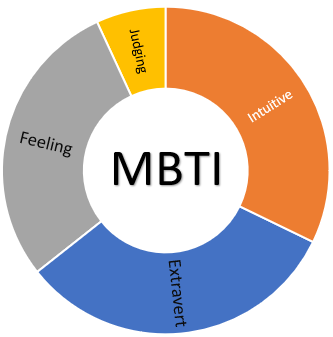
\includegraphics[scale=0.50]{img/MBTI.PNG}
    ~
 \section{Languages}
    \textbf{English}
\includegraphics[scale=0.40]{img/5stars.png}
    \textbf{Hindi}
\includegraphics[scale=0.40]{img/5stars.png}
    \textbf{Bengali}
\includegraphics[scale=0.40]{img/5stars.png}
    \textbf{Marathi}
\includegraphics[scale=0.40]{img/2stars.png}
    


\end{aside}

\section{Experience}
\begin{entrylist}
  \entry
    {07/17 - Now}
    {Product Consultant}
    {Nielsen+Partner, Singapore}
    {\emph{Temenos' Triple A Plus and WealthSuite Stack}\\
    Consulted for Bank of Singapore in enhancing their Triple A Plus implementation. Improved their interface solutions (Unix) and Web User Interface (WUI) components, based on business needs. Automated the validation of trade data between the host system and Triple A Plus for the generation of monthly client statements\\\emph{Promoted from Junior Consultant to Consultant}}
  \entry
    {11/16 - 04/17}
    {Intern Developer \& Data Analyst}
    {Singapore Exchange, Singapore}
    {Designed and developed Web based dashboards using appropriate "Visual Analytics" concepts.They enabled business users to use trading insights in day to day operations\\}
    \entry
    {01/16 - 04/17}
    {Space Technology Engineer}
    {Bhattacharya Space Enterprises (start-up), Singapore}
    {Spearheaded the company's first project with Singapore American School which sent Singapore's first fully automated experiment to the International Space Station\\}
    \entry
    {06/15 - 06/16}
    {Process Engineer}
    {Philips Lumileds, Singapore}
    {Maintained and improved the lithography and etch processes critical in the fabrication of High Brightness LEDs used as Smartphone flashlights.\\}
    \entry
    {05/15 - 12/15}
    {Project Partner}
    {Haku (start-up), Singapore}
    {Managed a team of university interns to execute sales, online brand management, and innovative, assessment center styled career fairs to connect recent graduates and mid-tier SMEs\\}
    \entry
    {07/12 - 07/14}
    {Undergraduate Internships}
    {Singapore, Germany}
    {Product testing intern at Autodesk for their AutoCad release.\\
    LED characterizing Intern at the photonics department of Humboldt University of Berlin.\\
    Organic Photovoltaic Intern at A*Star Institute of Materials Research and Engineering Singapore}
\end{entrylist}

\section{Education}
\begin{entrylist}
  \entry
    {2016 - 2017}
    {Master of IT in Business Analytics}
    {Singapore Management University, Singapore}
    {Focus on Data Analytics.\\
    Main subjects: Data Anlaytics Methods, Big Data, Visual Analytics, Banking Enterprise Architecture, IT Project Management, Strategy and Organisation\\}
    
  \entry
    {2011 - 2015}
    {B.Eng in Engineering Science}
    {National University of Singapore, Singapore}
    {Specialisation: Photonics and Optics\\
    \emph{Title of the Thesis: "Optical Collector Design Exploration of an Infrared Imager for a microsatellite aimed at Detecting and Locating High Temperature Events around the Singaporean and Indonesian Archipelago.".}}

\end{entrylist}
\newpage
\begin{aside}
\section{Volunteering}
    Aidha Mentor for computer skills
    Singapore
\end{aside}

\section{Certifications}
\begin{entrylist}
 \entry
 {2018}
    {Introduction to SQL}
    {Michigan University, Coursera}
    {\emph{Certification taken to build hobby projects in PHP}}
 \entry
    {2018}
    {Building Web Applications in PHP}
    {Michigan University, Coursera}
    {\emph{Certification taken to build hobby projects in PHP}}
  \entry
    {2015}
    {Digital Branding And Engagement}
    {Curtin University, EDX}
    {\emph{Digital Branding for application in Start-Ups}}
  \entry
    {2012 -2015}
    {Satellite Systems Design}
    {National University of Singapore, Design Centric Program}
    {\emph{Developing Satellite Systems}}
 
    
\end{entrylist}

\end{document}
